\documentclass[twoside]{book}

% Packages required by doxygen
\usepackage{fixltx2e}
\usepackage{calc}
\usepackage{doxygen}
\usepackage[export]{adjustbox} % also loads graphicx
\usepackage{graphicx}
\usepackage[utf8]{inputenc}
\usepackage{makeidx}
\usepackage{multicol}
\usepackage{multirow}
\PassOptionsToPackage{warn}{textcomp}
\usepackage{textcomp}
\usepackage[nointegrals]{wasysym}
\usepackage[table]{xcolor}

% Font selection
\usepackage[T1]{fontenc}
\usepackage[scaled=.90]{helvet}
\usepackage{courier}
\usepackage{amssymb}
\usepackage{sectsty}
\renewcommand{\familydefault}{\sfdefault}
\allsectionsfont{%
  \fontseries{bc}\selectfont%
  \color{darkgray}%
}
\renewcommand{\DoxyLabelFont}{%
  \fontseries{bc}\selectfont%
  \color{darkgray}%
}
\newcommand{\+}{\discretionary{\mbox{\scriptsize$\hookleftarrow$}}{}{}}

% Page & text layout
\usepackage{geometry}
\geometry{%
  a4paper,%
  top=2.5cm,%
  bottom=2.5cm,%
  left=2.5cm,%
  right=2.5cm%
}
\tolerance=750
\hfuzz=15pt
\hbadness=750
\setlength{\emergencystretch}{15pt}
\setlength{\parindent}{0cm}
\setlength{\parskip}{3ex plus 2ex minus 2ex}
\makeatletter
\renewcommand{\paragraph}{%
  \@startsection{paragraph}{4}{0ex}{-1.0ex}{1.0ex}{%
    \normalfont\normalsize\bfseries\SS@parafont%
  }%
}
\renewcommand{\subparagraph}{%
  \@startsection{subparagraph}{5}{0ex}{-1.0ex}{1.0ex}{%
    \normalfont\normalsize\bfseries\SS@subparafont%
  }%
}
\makeatother

% Headers & footers
\usepackage{fancyhdr}
\pagestyle{fancyplain}
\fancyhead[LE]{\fancyplain{}{\bfseries\thepage}}
\fancyhead[CE]{\fancyplain{}{}}
\fancyhead[RE]{\fancyplain{}{\bfseries\leftmark}}
\fancyhead[LO]{\fancyplain{}{\bfseries\rightmark}}
\fancyhead[CO]{\fancyplain{}{}}
\fancyhead[RO]{\fancyplain{}{\bfseries\thepage}}
\fancyfoot[LE]{\fancyplain{}{}}
\fancyfoot[CE]{\fancyplain{}{}}
\fancyfoot[RE]{\fancyplain{}{\bfseries\scriptsize Generated by Doxygen }}
\fancyfoot[LO]{\fancyplain{}{\bfseries\scriptsize Generated by Doxygen }}
\fancyfoot[CO]{\fancyplain{}{}}
\fancyfoot[RO]{\fancyplain{}{}}
\renewcommand{\footrulewidth}{0.4pt}
\renewcommand{\chaptermark}[1]{%
  \markboth{#1}{}%
}
\renewcommand{\sectionmark}[1]{%
  \markright{\thesection\ #1}%
}

% Indices & bibliography
\usepackage{natbib}
\usepackage[titles]{tocloft}
\setcounter{tocdepth}{3}
\setcounter{secnumdepth}{5}
\makeindex

% Hyperlinks (required, but should be loaded last)
\usepackage{ifpdf}
\ifpdf
  \usepackage[pdftex,pagebackref=true]{hyperref}
\else
  \usepackage[ps2pdf,pagebackref=true]{hyperref}
\fi
\hypersetup{%
  colorlinks=true,%
  linkcolor=blue,%
  citecolor=blue,%
  unicode%
}

% Custom commands
\newcommand{\clearemptydoublepage}{%
  \newpage{\pagestyle{empty}\cleardoublepage}%
}

\usepackage{caption}
\captionsetup{labelsep=space,justification=centering,font={bf},singlelinecheck=off,skip=4pt,position=top}

%===== C O N T E N T S =====

\begin{document}

% Titlepage & ToC
\hypersetup{pageanchor=false,
             bookmarksnumbered=true,
             pdfencoding=unicode
            }
\pagenumbering{alph}
\begin{titlepage}
\vspace*{7cm}
\begin{center}%
{\Large yaml\+\_\+cpp\+\_\+catkin }\\
\vspace*{1cm}
{\large Generated by Doxygen 1.8.13}\\
\end{center}
\end{titlepage}
\clearemptydoublepage
\pagenumbering{roman}
\tableofcontents
\clearemptydoublepage
\pagenumbering{arabic}
\hypersetup{pageanchor=true}

%--- Begin generated contents ---
\chapter{License}
\label{license}
\Hypertarget{license}

\begin{DoxyRefList}
\item[\label{license__license000001}%
\Hypertarget{license__license000001}%
File \hyperlink{yaml__cpp__fwd_8hpp}{yaml\+\_\+cpp\+\_\+fwd.hpp} ]License B\+S\+D-\/3-\/\+Clause  
\item[\label{license__license000002}%
\Hypertarget{license__license000002}%
File \hyperlink{yaml__eigen_8h}{yaml\+\_\+eigen.h} ]License B\+S\+D-\/3-\/\+Clause  
\item[\label{license__license000003}%
\Hypertarget{license__license000003}%
File \hyperlink{yaml__tools_8hpp}{yaml\+\_\+tools.hpp} ]License B\+S\+D-\/3-\/\+Clause 
\end{DoxyRefList}
\chapter{Class Index}
\section{Class List}
Here are the classes, structs, unions and interfaces with brief descriptions\+:\begin{DoxyCompactList}
\item\contentsline{section}{\hyperlink{classshared__memory_1_1Allocation__exception}{shared\+\_\+memory\+::\+Allocation\+\_\+exception} }{\pageref{classshared__memory_1_1Allocation__exception}}{}
\item\contentsline{section}{\hyperlink{classshared__memory_1_1array}{shared\+\_\+memory\+::array$<$ T, S\+I\+Z\+E $>$} \\*Implement a shared array stored on a shared memory segment }{\pageref{classshared__memory_1_1array}}{}
\item\contentsline{section}{\hyperlink{classshared__memory_1_1internal_1_1array__members}{shared\+\_\+memory\+::internal\+::array\+\_\+members$<$ T, S\+I\+Z\+E, Enable $>$} }{\pageref{classshared__memory_1_1internal_1_1array__members}}{}
\item\contentsline{section}{\hyperlink{classshared__memory_1_1internal_1_1array__members_3_01T_00_010_00_01typename_01std_1_1enable__ifb2fde5f96702510d664610c5e9570772}{shared\+\_\+memory\+::internal\+::array\+\_\+members$<$ T, 0, typename std\+::enable\+\_\+if$<$ std\+::is\+\_\+fundamental$<$ T $>$\+::value $>$\+::type $>$} }{\pageref{classshared__memory_1_1internal_1_1array__members_3_01T_00_010_00_01typename_01std_1_1enable__ifb2fde5f96702510d664610c5e9570772}}{}
\item\contentsline{section}{\hyperlink{classshared__memory_1_1internal_1_1array__members_3_01T_00_01SIZE_00_01typename_01std_1_1enable_de9984c52d14535c26d7a424fbd87fe2}{shared\+\_\+memory\+::internal\+::array\+\_\+members$<$ T, S\+I\+Z\+E, typename std\+::enable\+\_\+if$<$ std\+::is\+\_\+fundamental$<$ T $>$\+::value \&\&\+S\+I\+Z\+E!=0 $>$\+::type $>$} }{\pageref{classshared__memory_1_1internal_1_1array__members_3_01T_00_01SIZE_00_01typename_01std_1_1enable_de9984c52d14535c26d7a424fbd87fe2}}{}
\item\contentsline{section}{\hyperlink{classshared__memory_1_1ConditionVariable}{shared\+\_\+memory\+::\+Condition\+Variable} }{\pageref{classshared__memory_1_1ConditionVariable}}{}
\item\contentsline{section}{\hyperlink{classConfig}{Config} }{\pageref{classConfig}}{}
\item\contentsline{section}{\hyperlink{classshared__memory_1_1Exchange__manager__consumer}{shared\+\_\+memory\+::\+Exchange\+\_\+manager\+\_\+consumer$<$ Serializable, Q\+U\+E\+U\+E\+\_\+\+S\+I\+Z\+E $>$} }{\pageref{classshared__memory_1_1Exchange__manager__consumer}}{}
\item\contentsline{section}{\hyperlink{classshared__memory_1_1internal_1_1Exchange__manager__memory}{shared\+\_\+memory\+::internal\+::\+Exchange\+\_\+manager\+\_\+memory$<$ Serializable, Q\+U\+E\+U\+E\+\_\+\+S\+I\+Z\+E $>$} }{\pageref{classshared__memory_1_1internal_1_1Exchange__manager__memory}}{}
\item\contentsline{section}{\hyperlink{classshared__memory_1_1Exchange__manager__producer}{shared\+\_\+memory\+::\+Exchange\+\_\+manager\+\_\+producer$<$ Serializable, Q\+U\+E\+U\+E\+\_\+\+S\+I\+Z\+E $>$} }{\pageref{classshared__memory_1_1Exchange__manager__producer}}{}
\item\contentsline{section}{\hyperlink{classshared__memory_1_1Four__int__values}{shared\+\_\+memory\+::\+Four\+\_\+int\+\_\+values} \\*Example of an instance that can be serialized }{\pageref{classshared__memory_1_1Four__int__values}}{}
\item\contentsline{section}{\hyperlink{classshared__memory_1_1Item}{shared\+\_\+memory\+::\+Item$<$ S\+I\+Z\+E $>$} }{\pageref{classshared__memory_1_1Item}}{}
\item\contentsline{section}{\hyperlink{classshared__memory_1_1Lock}{shared\+\_\+memory\+::\+Lock} \\*A scope lock object for locking a shared memory mutex, to use for example with a shared memory condition variable }{\pageref{classshared__memory_1_1Lock}}{}
\item\contentsline{section}{\hyperlink{classshared__memory_1_1LockedConditionVariable}{shared\+\_\+memory\+::\+Locked\+Condition\+Variable} \\*Here as a anonymous layer on top of the boost intersprocess condition variable labrary }{\pageref{classshared__memory_1_1LockedConditionVariable}}{}
\item\contentsline{section}{\hyperlink{structMeasureTime}{Measure\+Time} }{\pageref{structMeasureTime}}{}
\item\contentsline{section}{\hyperlink{classshared__memory_1_1Memory__overflow__exception}{shared\+\_\+memory\+::\+Memory\+\_\+overflow\+\_\+exception} }{\pageref{classshared__memory_1_1Memory__overflow__exception}}{}
\item\contentsline{section}{\hyperlink{classshared__memory_1_1Mutex}{shared\+\_\+memory\+::\+Mutex} }{\pageref{classshared__memory_1_1Mutex}}{}
\item\contentsline{section}{\hyperlink{classshared__memory_1_1Not__consumed__exception}{shared\+\_\+memory\+::\+Not\+\_\+consumed\+\_\+exception} }{\pageref{classshared__memory_1_1Not__consumed__exception}}{}
\item\contentsline{section}{\hyperlink{classshared__memory_1_1SegmentInfo}{shared\+\_\+memory\+::\+Segment\+Info} \\*Encapsulate information related to a shared memory segment }{\pageref{classshared__memory_1_1SegmentInfo}}{}
\item\contentsline{section}{\hyperlink{classSerializable}{Serializable$<$ S\+I\+Z\+E $>$} }{\pageref{classSerializable}}{}
\item\contentsline{section}{\hyperlink{classshared__memory_1_1Serializable__exchange}{shared\+\_\+memory\+::\+Serializable\+\_\+exchange$<$ Serializable $>$} }{\pageref{classshared__memory_1_1Serializable__exchange}}{}
\item\contentsline{section}{\hyperlink{classSerializableExample}{Serializable\+Example} }{\pageref{classSerializableExample}}{}
\item\contentsline{section}{\hyperlink{classshared__memory_1_1internal_1_1Serialized__read}{shared\+\_\+memory\+::internal\+::\+Serialized\+\_\+read$<$ Serializable $>$} }{\pageref{classshared__memory_1_1internal_1_1Serialized__read}}{}
\item\contentsline{section}{\hyperlink{classshared__memory_1_1internal_1_1Serialized__write}{shared\+\_\+memory\+::internal\+::\+Serialized\+\_\+write$<$ Serializable $>$} }{\pageref{classshared__memory_1_1internal_1_1Serialized__write}}{}
\item\contentsline{section}{\hyperlink{classshared__memory_1_1Serializer}{shared\+\_\+memory\+::\+Serializer$<$ Serializable $>$} }{\pageref{classshared__memory_1_1Serializer}}{}
\item\contentsline{section}{\hyperlink{classshared__memory_1_1SharedMemorySegment}{shared\+\_\+memory\+::\+Shared\+Memory\+Segment} \\*The \hyperlink{classshared__memory_1_1SharedMemorySegment}{Shared\+Memory\+Segment} contains the pointers of the shared objects in on shared memrory segment }{\pageref{classshared__memory_1_1SharedMemorySegment}}{}
\item\contentsline{section}{\hyperlink{structshared__memory_1_1ShmTypeHelper}{shared\+\_\+memory\+::\+Shm\+Type\+Helper$<$ Elem\+Type $>$} \\*\hyperlink{structshared__memory_1_1ShmTypeHelper}{Shm\+Type\+Helper} is a small struct that allow the definition of templated typedef }{\pageref{structshared__memory_1_1ShmTypeHelper}}{}
\item\contentsline{section}{\hyperlink{classshared__memory_1_1Unexpected__map__key}{shared\+\_\+memory\+::\+Unexpected\+\_\+map\+\_\+key$<$ Key $>$} }{\pageref{classshared__memory_1_1Unexpected__map__key}}{}
\item\contentsline{section}{\hyperlink{classshared__memory_1_1Unexpected__size__exception}{shared\+\_\+memory\+::\+Unexpected\+\_\+size\+\_\+exception} }{\pageref{classshared__memory_1_1Unexpected__size__exception}}{}
\end{DoxyCompactList}

\chapter{File Index}
\section{File List}
Here is a list of all documented files with brief descriptions\+:\begin{DoxyCompactList}
\item\contentsline{section}{include/dg\+\_\+blmc\+\_\+robots/\hyperlink{common__header_8hpp}{common\+\_\+header.\+hpp} }{\pageref{common__header_8hpp}}{}
\item\contentsline{section}{include/dg\+\_\+blmc\+\_\+robots/\hyperlink{dgm__single__motor_8hpp}{dgm\+\_\+single\+\_\+motor.\+hpp} }{\pageref{dgm__single__motor_8hpp}}{}
\item\contentsline{section}{include/dg\+\_\+blmc\+\_\+robots/{\bfseries dgm\+\_\+solo12.\+hpp} }{\pageref{dgm__solo12_8hpp}}{}
\item\contentsline{section}{include/dg\+\_\+blmc\+\_\+robots/{\bfseries dgm\+\_\+solo8.\+hpp} }{\pageref{dgm__solo8_8hpp}}{}
\item\contentsline{section}{include/dg\+\_\+blmc\+\_\+robots/{\bfseries dgm\+\_\+solo8ti.\+hpp} }{\pageref{dgm__solo8ti_8hpp}}{}
\item\contentsline{section}{include/dg\+\_\+blmc\+\_\+robots/{\bfseries dgm\+\_\+solo\+\_\+simple\+\_\+simu.\+hpp} }{\pageref{dgm__solo__simple__simu_8hpp}}{}
\item\contentsline{section}{include/dg\+\_\+blmc\+\_\+robots/\hyperlink{dgm__stuggihop_8hpp}{dgm\+\_\+stuggihop.\+hpp} }{\pageref{dgm__stuggihop_8hpp}}{}
\item\contentsline{section}{include/dg\+\_\+blmc\+\_\+robots/{\bfseries dgm\+\_\+teststand.\+hpp} }{\pageref{dgm__teststand_8hpp}}{}
\item\contentsline{section}{src/\hyperlink{dgm__solo__simple__simu_8cpp}{dgm\+\_\+solo\+\_\+simple\+\_\+simu.\+cpp} \\*The hardware wrapper of the solo naive simulation }{\pageref{dgm__solo__simple__simu_8cpp}}{}
\item\contentsline{section}{src/\hyperlink{dgm__stuggihop_8cpp}{dgm\+\_\+stuggihop.\+cpp} \\*D\+GM wrapper around the stuggihop robot }{\pageref{dgm__stuggihop_8cpp}}{}
\end{DoxyCompactList}

\chapter{Class Documentation}
\hypertarget{structYAML_1_1convert_3_01Eigen_1_1Matrix_3_01Scalar_00_01Rows_00_01Cols_00_01Align_00_01RowsAtC8665abb6da4eb6935869b0ee422ba9ce}{}\section{Y\+A\+ML\+:\+:convert$<$ Eigen\+:\+:Matrix$<$ Scalar, Rows, Cols, Align, Rows\+At\+Compile\+Time, Cols\+At\+Compile\+Time $>$ $>$ Struct Template Reference}
\label{structYAML_1_1convert_3_01Eigen_1_1Matrix_3_01Scalar_00_01Rows_00_01Cols_00_01Align_00_01RowsAtC8665abb6da4eb6935869b0ee422ba9ce}\index{Y\+A\+M\+L\+::convert$<$ Eigen\+::\+Matrix$<$ Scalar, Rows, Cols, Align, Rows\+At\+Compile\+Time, Cols\+At\+Compile\+Time $>$ $>$@{Y\+A\+M\+L\+::convert$<$ Eigen\+::\+Matrix$<$ Scalar, Rows, Cols, Align, Rows\+At\+Compile\+Time, Cols\+At\+Compile\+Time $>$ $>$}}
\subsection*{Public Types}
\begin{DoxyCompactItemize}
\item 
\mbox{\Hypertarget{structYAML_1_1convert_3_01Eigen_1_1Matrix_3_01Scalar_00_01Rows_00_01Cols_00_01Align_00_01RowsAtC8665abb6da4eb6935869b0ee422ba9ce_a798e760d2b03324cecd1da2db5680c5a}\label{structYAML_1_1convert_3_01Eigen_1_1Matrix_3_01Scalar_00_01Rows_00_01Cols_00_01Align_00_01RowsAtC8665abb6da4eb6935869b0ee422ba9ce_a798e760d2b03324cecd1da2db5680c5a}} 
typedef Eigen\+::\+Matrix$<$ Scalar, Rows, Cols, Align, Rows\+At\+Compile\+Time, Cols\+At\+Compile\+Time $>$ {\bfseries Eigen\+\_\+\+Type\+\_\+}
\item 
\mbox{\Hypertarget{structYAML_1_1convert_3_01Eigen_1_1Matrix_3_01Scalar_00_01Rows_00_01Cols_00_01Align_00_01RowsAtC8665abb6da4eb6935869b0ee422ba9ce_a88ccaf7da608e0afffffd7248f54b75a}\label{structYAML_1_1convert_3_01Eigen_1_1Matrix_3_01Scalar_00_01Rows_00_01Cols_00_01Align_00_01RowsAtC8665abb6da4eb6935869b0ee422ba9ce_a88ccaf7da608e0afffffd7248f54b75a}} 
typedef std\+::conditional$<$ is\+\_\+vector\+\_\+type\+\_\+, \hyperlink{structYAML_1_1EigenVectorConverter}{Eigen\+Vector\+Converter}$<$ Scalar, Rows, Cols, Align, Rows\+At\+Compile\+Time, Cols\+At\+Compile\+Time $>$, \hyperlink{structYAML_1_1EigenMatrixConverter}{Eigen\+Matrix\+Converter}$<$ Scalar, Rows, Cols, Align, Rows\+At\+Compile\+Time, Cols\+At\+Compile\+Time $>$ $>$\+::type {\bfseries Converter\+\_\+}
\end{DoxyCompactItemize}
\subsection*{Static Public Member Functions}
\begin{DoxyCompactItemize}
\item 
\mbox{\Hypertarget{structYAML_1_1convert_3_01Eigen_1_1Matrix_3_01Scalar_00_01Rows_00_01Cols_00_01Align_00_01RowsAtC8665abb6da4eb6935869b0ee422ba9ce_ab1716b1cd1af6ef1bdb89dd867b05dc6}\label{structYAML_1_1convert_3_01Eigen_1_1Matrix_3_01Scalar_00_01Rows_00_01Cols_00_01Align_00_01RowsAtC8665abb6da4eb6935869b0ee422ba9ce_ab1716b1cd1af6ef1bdb89dd867b05dc6}} 
static Node {\bfseries encode} (const Eigen\+\_\+\+Type\+\_\+ \&rhs)
\item 
\mbox{\Hypertarget{structYAML_1_1convert_3_01Eigen_1_1Matrix_3_01Scalar_00_01Rows_00_01Cols_00_01Align_00_01RowsAtC8665abb6da4eb6935869b0ee422ba9ce_a27f60d49bf29a84c2d3e14a52e12df65}\label{structYAML_1_1convert_3_01Eigen_1_1Matrix_3_01Scalar_00_01Rows_00_01Cols_00_01Align_00_01RowsAtC8665abb6da4eb6935869b0ee422ba9ce_a27f60d49bf29a84c2d3e14a52e12df65}} 
static bool {\bfseries decode\+\_\+2d} (const Node \&node, Eigen\+\_\+\+Type\+\_\+ \&rhs)
\item 
\mbox{\Hypertarget{structYAML_1_1convert_3_01Eigen_1_1Matrix_3_01Scalar_00_01Rows_00_01Cols_00_01Align_00_01RowsAtC8665abb6da4eb6935869b0ee422ba9ce_a596a49e214c2b493de23185ca5d7ff38}\label{structYAML_1_1convert_3_01Eigen_1_1Matrix_3_01Scalar_00_01Rows_00_01Cols_00_01Align_00_01RowsAtC8665abb6da4eb6935869b0ee422ba9ce_a596a49e214c2b493de23185ca5d7ff38}} 
static bool {\bfseries decode\+\_\+1d} (const Node \&node, Eigen\+\_\+\+Type\+\_\+ \&rhs)
\item 
\mbox{\Hypertarget{structYAML_1_1convert_3_01Eigen_1_1Matrix_3_01Scalar_00_01Rows_00_01Cols_00_01Align_00_01RowsAtC8665abb6da4eb6935869b0ee422ba9ce_ab8738e33c1392218faf566a1e75395e4}\label{structYAML_1_1convert_3_01Eigen_1_1Matrix_3_01Scalar_00_01Rows_00_01Cols_00_01Align_00_01RowsAtC8665abb6da4eb6935869b0ee422ba9ce_ab8738e33c1392218faf566a1e75395e4}} 
static bool {\bfseries decode} (const Node \&node, Eigen\+\_\+\+Type\+\_\+ \&rhs)
\end{DoxyCompactItemize}
\subsection*{Static Public Attributes}
\begin{DoxyCompactItemize}
\item 
\mbox{\Hypertarget{structYAML_1_1convert_3_01Eigen_1_1Matrix_3_01Scalar_00_01Rows_00_01Cols_00_01Align_00_01RowsAtC8665abb6da4eb6935869b0ee422ba9ce_a02420fa6ad9be337bfcdbb83f7c292c3}\label{structYAML_1_1convert_3_01Eigen_1_1Matrix_3_01Scalar_00_01Rows_00_01Cols_00_01Align_00_01RowsAtC8665abb6da4eb6935869b0ee422ba9ce_a02420fa6ad9be337bfcdbb83f7c292c3}} 
static const bool {\bfseries is\+\_\+vector\+\_\+type\+\_\+} = Rows == 1 $\vert$$\vert$ Cols == 1
\end{DoxyCompactItemize}


The documentation for this struct was generated from the following file\+:\begin{DoxyCompactItemize}
\item 
include/yaml\+\_\+cpp\+\_\+catkin/\hyperlink{yaml__eigen_8h}{yaml\+\_\+eigen.\+h}\end{DoxyCompactItemize}

\hypertarget{structYAML_1_1convert_3_01Eigen_1_1Quaterniond_01_4}{}\section{Y\+A\+ML\+:\+:convert$<$ Eigen\+:\+:Quaterniond $>$ Struct Template Reference}
\label{structYAML_1_1convert_3_01Eigen_1_1Quaterniond_01_4}\index{Y\+A\+M\+L\+::convert$<$ Eigen\+::\+Quaterniond $>$@{Y\+A\+M\+L\+::convert$<$ Eigen\+::\+Quaterniond $>$}}
\subsection*{Static Public Member Functions}
\begin{DoxyCompactItemize}
\item 
static Node {\bfseries encode} (const Eigen\+::\+Quaterniond \&mp)\hypertarget{structYAML_1_1convert_3_01Eigen_1_1Quaterniond_01_4_a85181ea20e6b7dc21b6daffa53d745ee}{}\label{structYAML_1_1convert_3_01Eigen_1_1Quaterniond_01_4_a85181ea20e6b7dc21b6daffa53d745ee}

\item 
static bool {\bfseries decode} (const Node \&node, Eigen\+::\+Quaterniond \&mp)\hypertarget{structYAML_1_1convert_3_01Eigen_1_1Quaterniond_01_4_add796e15f8e6672ada052f112cbf3f51}{}\label{structYAML_1_1convert_3_01Eigen_1_1Quaterniond_01_4_add796e15f8e6672ada052f112cbf3f51}

\end{DoxyCompactItemize}


The documentation for this struct was generated from the following file\+:\begin{DoxyCompactItemize}
\item 
include/yaml\+\_\+cpp\+\_\+catkin/\hyperlink{yaml__eigen_8h}{yaml\+\_\+eigen.\+h}\end{DoxyCompactItemize}

\hypertarget{structYAML_1_1convert_3_01robot__math_1_1MovableEigenVector_3_01T_01_4_01_4}{}\section{Y\+A\+ML\+:\+:convert$<$ robot\+\_\+math\+:\+:Movable\+Eigen\+Vector$<$ T $>$ $>$ Struct Template Reference}
\label{structYAML_1_1convert_3_01robot__math_1_1MovableEigenVector_3_01T_01_4_01_4}\index{Y\+A\+M\+L\+::convert$<$ robot\+\_\+math\+::\+Movable\+Eigen\+Vector$<$ T $>$ $>$@{Y\+A\+M\+L\+::convert$<$ robot\+\_\+math\+::\+Movable\+Eigen\+Vector$<$ T $>$ $>$}}
\subsection*{Static Public Member Functions}
\begin{DoxyCompactItemize}
\item 
\mbox{\Hypertarget{structYAML_1_1convert_3_01robot__math_1_1MovableEigenVector_3_01T_01_4_01_4_a1eaba2e3451344a859914e8a781d542e}\label{structYAML_1_1convert_3_01robot__math_1_1MovableEigenVector_3_01T_01_4_01_4_a1eaba2e3451344a859914e8a781d542e}} 
static Node {\bfseries encode} (const \hyperlink{structrobot__math_1_1MovableEigenVector}{robot\+\_\+math\+::\+Movable\+Eigen\+Vector}$<$ T $>$ \&mp)
\item 
\mbox{\Hypertarget{structYAML_1_1convert_3_01robot__math_1_1MovableEigenVector_3_01T_01_4_01_4_a31a0b4061fd234b46a046cb9f87994f2}\label{structYAML_1_1convert_3_01robot__math_1_1MovableEigenVector_3_01T_01_4_01_4_a31a0b4061fd234b46a046cb9f87994f2}} 
static bool {\bfseries decode} (const Node \&node, \hyperlink{structrobot__math_1_1MovableEigenVector}{robot\+\_\+math\+::\+Movable\+Eigen\+Vector}$<$ T $>$ \&mp)
\end{DoxyCompactItemize}


The documentation for this struct was generated from the following file\+:\begin{DoxyCompactItemize}
\item 
include/yaml\+\_\+cpp\+\_\+catkin/\hyperlink{yaml__eigen_8h}{yaml\+\_\+eigen.\+h}\end{DoxyCompactItemize}

\hypertarget{structYAML_1_1EigenMatrixConverter}{}\section{Y\+A\+ML\+:\+:Eigen\+Matrix\+Converter$<$ Scalar, Rows, Cols, Align, Rows\+At\+Compile\+Time, Cols\+At\+Compile\+Time $>$ Struct Template Reference}
\label{structYAML_1_1EigenMatrixConverter}\index{Y\+A\+M\+L\+::\+Eigen\+Matrix\+Converter$<$ Scalar, Rows, Cols, Align, Rows\+At\+Compile\+Time, Cols\+At\+Compile\+Time $>$@{Y\+A\+M\+L\+::\+Eigen\+Matrix\+Converter$<$ Scalar, Rows, Cols, Align, Rows\+At\+Compile\+Time, Cols\+At\+Compile\+Time $>$}}
\subsection*{Public Types}
\begin{DoxyCompactItemize}
\item 
\mbox{\Hypertarget{structYAML_1_1EigenMatrixConverter_a46c2e1524d0287ef8e0bbfad07f4111a}\label{structYAML_1_1EigenMatrixConverter_a46c2e1524d0287ef8e0bbfad07f4111a}} 
typedef Eigen\+::\+Matrix$<$ Scalar, Rows, Cols, Align, Rows\+At\+Compile\+Time, Cols\+At\+Compile\+Time $>$ {\bfseries Matrix\+Type}
\end{DoxyCompactItemize}
\subsection*{Static Public Member Functions}
\begin{DoxyCompactItemize}
\item 
\mbox{\Hypertarget{structYAML_1_1EigenMatrixConverter_a61d62ab23d2ff9fe961f052e18da4998}\label{structYAML_1_1EigenMatrixConverter_a61d62ab23d2ff9fe961f052e18da4998}} 
static void {\bfseries resize\+\_\+if\+\_\+needed} (int rows, int cols, Matrix\+Type \&rhs)
\item 
\mbox{\Hypertarget{structYAML_1_1EigenMatrixConverter_ad9f58bba84fc000b6aecd10142ecc16e}\label{structYAML_1_1EigenMatrixConverter_ad9f58bba84fc000b6aecd10142ecc16e}} 
static Scalar \& {\bfseries access\+\_\+element} (int r, int c, Matrix\+Type \&rhs)
\end{DoxyCompactItemize}


The documentation for this struct was generated from the following file\+:\begin{DoxyCompactItemize}
\item 
include/yaml\+\_\+cpp\+\_\+catkin/\hyperlink{yaml__eigen_8h}{yaml\+\_\+eigen.\+h}\end{DoxyCompactItemize}

\hypertarget{structYAML_1_1EigenVectorConverter}{}\section{Y\+A\+ML\+:\+:Eigen\+Vector\+Converter$<$ Scalar, Rows, Cols, Align, Rows\+At\+Compile\+Time, Cols\+At\+Compile\+Time $>$ Struct Template Reference}
\label{structYAML_1_1EigenVectorConverter}\index{Y\+A\+M\+L\+::\+Eigen\+Vector\+Converter$<$ Scalar, Rows, Cols, Align, Rows\+At\+Compile\+Time, Cols\+At\+Compile\+Time $>$@{Y\+A\+M\+L\+::\+Eigen\+Vector\+Converter$<$ Scalar, Rows, Cols, Align, Rows\+At\+Compile\+Time, Cols\+At\+Compile\+Time $>$}}
\subsection*{Public Types}
\begin{DoxyCompactItemize}
\item 
typedef Eigen\+::\+Matrix$<$ Scalar, Rows, Cols, Align, Rows\+At\+Compile\+Time, Cols\+At\+Compile\+Time $>$ {\bfseries Vector\+Type}\hypertarget{structYAML_1_1EigenVectorConverter_afa182cb98f58630ff1ed5548a961474e}{}\label{structYAML_1_1EigenVectorConverter_afa182cb98f58630ff1ed5548a961474e}

\end{DoxyCompactItemize}
\subsection*{Static Public Member Functions}
\begin{DoxyCompactItemize}
\item 
static void {\bfseries resize\+\_\+if\+\_\+needed} (int rows, int cols, Vector\+Type \&rhs)\hypertarget{structYAML_1_1EigenVectorConverter_a7a791e9412c2386c59b33794d7bd339a}{}\label{structYAML_1_1EigenVectorConverter_a7a791e9412c2386c59b33794d7bd339a}

\item 
static Scalar \& {\bfseries access\+\_\+element} (int r, int c, Vector\+Type \&rhs)\hypertarget{structYAML_1_1EigenVectorConverter_a6d52c444a505118006dc1e721da15fad}{}\label{structYAML_1_1EigenVectorConverter_a6d52c444a505118006dc1e721da15fad}

\end{DoxyCompactItemize}


The documentation for this struct was generated from the following file\+:\begin{DoxyCompactItemize}
\item 
include/yaml\+\_\+cpp\+\_\+catkin/\hyperlink{yaml__eigen_8h}{yaml\+\_\+eigen.\+h}\end{DoxyCompactItemize}

\hypertarget{structrobot__math_1_1MovableEigenMatrix}{}\section{robot\+\_\+math\+:\+:Movable\+Eigen\+Matrix$<$ T $>$ Struct Template Reference}
\label{structrobot__math_1_1MovableEigenMatrix}\index{robot\+\_\+math\+::\+Movable\+Eigen\+Matrix$<$ T $>$@{robot\+\_\+math\+::\+Movable\+Eigen\+Matrix$<$ T $>$}}


The documentation for this struct was generated from the following file\+:\begin{DoxyCompactItemize}
\item 
include/yaml\+\_\+cpp\+\_\+catkin/\hyperlink{yaml__eigen_8h}{yaml\+\_\+eigen.\+h}\end{DoxyCompactItemize}

\hypertarget{structrobot__math_1_1MovableEigenVector}{}\section{robot\+\_\+math\+:\+:Movable\+Eigen\+Vector$<$ T $>$ Struct Template Reference}
\label{structrobot__math_1_1MovableEigenVector}\index{robot\+\_\+math\+::\+Movable\+Eigen\+Vector$<$ T $>$@{robot\+\_\+math\+::\+Movable\+Eigen\+Vector$<$ T $>$}}


The documentation for this struct was generated from the following file\+:\begin{DoxyCompactItemize}
\item 
include/yaml\+\_\+cpp\+\_\+catkin/\hyperlink{yaml__eigen_8h}{yaml\+\_\+eigen.\+h}\end{DoxyCompactItemize}

\chapter{File Documentation}
\hypertarget{yaml__cpp__fwd_8hpp}{}\section{include/yaml\+\_\+cpp\+\_\+catkin/yaml\+\_\+cpp\+\_\+fwd.hpp File Reference}
\label{yaml__cpp__fwd_8hpp}\index{include/yaml\+\_\+cpp\+\_\+catkin/yaml\+\_\+cpp\+\_\+fwd.\+hpp@{include/yaml\+\_\+cpp\+\_\+catkin/yaml\+\_\+cpp\+\_\+fwd.\+hpp}}
{\ttfamily \#include $<$yaml-\/cpp/yaml.\+h$>$}\\*
{\ttfamily \#include \char`\"{}yaml\+\_\+cpp\+\_\+catkin/yaml\+\_\+eigen.\+h\char`\"{}}\\*
{\ttfamily \#include \char`\"{}yaml\+\_\+cpp\+\_\+catkin/yaml\+\_\+tools.\+hpp\char`\"{}}\\*
Include dependency graph for yaml\+\_\+cpp\+\_\+fwd.\+hpp\+:
\nopagebreak
\begin{figure}[H]
\begin{center}
\leavevmode
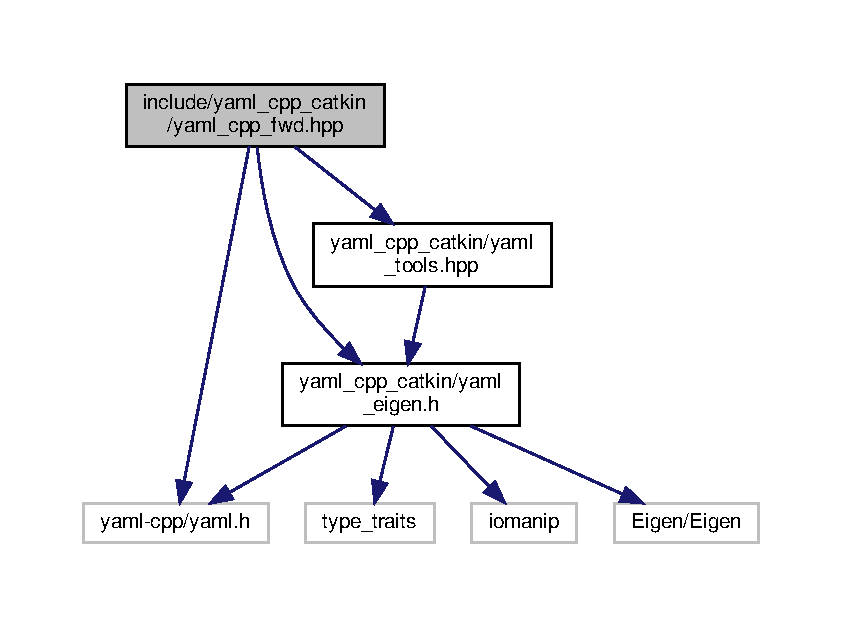
\includegraphics[width=350pt]{yaml__cpp__fwd_8hpp__incl}
\end{center}
\end{figure}


\subsection{Detailed Description}
\begin{DoxyAuthor}{Author}
Maximilien Naveau (\href{mailto:maximilien.naveau@gmail.com}{\tt maximilien.\+naveau@gmail.\+com}) 
\end{DoxyAuthor}
\begin{DoxyRefDesc}{License}
\item[\hyperlink{license__license000001}{License}]License B\+S\+D-\/3-\/\+Clause \end{DoxyRefDesc}
\begin{DoxyCopyright}{Copyright}
Copyright (c) 2019, New York University and Max Planck Gesellschaft. 
\end{DoxyCopyright}
\begin{DoxyDate}{Date}
2019-\/09-\/30 
\end{DoxyDate}

\hypertarget{yaml__eigen_8h}{}\section{include/yaml\+\_\+cpp\+\_\+catkin/yaml\+\_\+eigen.h File Reference}
\label{yaml__eigen_8h}\index{include/yaml\+\_\+cpp\+\_\+catkin/yaml\+\_\+eigen.\+h@{include/yaml\+\_\+cpp\+\_\+catkin/yaml\+\_\+eigen.\+h}}


Add support for eigen frm the yaml-\/cpp standard package.  


{\ttfamily \#include $<$type\+\_\+traits$>$}\newline
{\ttfamily \#include $<$iomanip$>$}\newline
{\ttfamily \#include $<$Eigen/\+Eigen$>$}\newline
{\ttfamily \#include $<$yaml-\/cpp/yaml.\+h$>$}\newline
Include dependency graph for yaml\+\_\+eigen.\+h\+:
\nopagebreak
\begin{figure}[H]
\begin{center}
\leavevmode
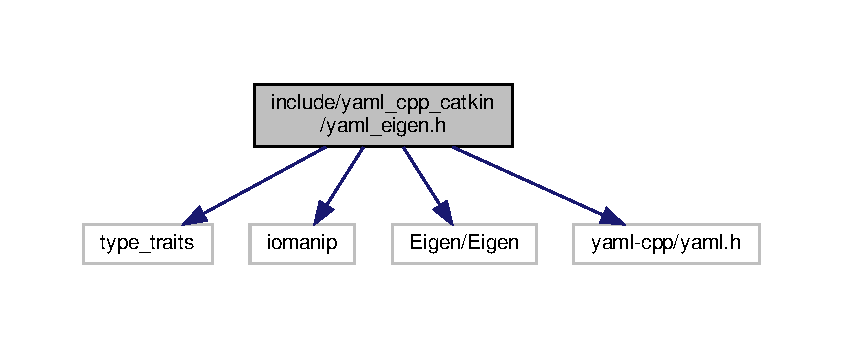
\includegraphics[width=350pt]{yaml__eigen_8h__incl}
\end{center}
\end{figure}
This graph shows which files directly or indirectly include this file\+:
\nopagebreak
\begin{figure}[H]
\begin{center}
\leavevmode
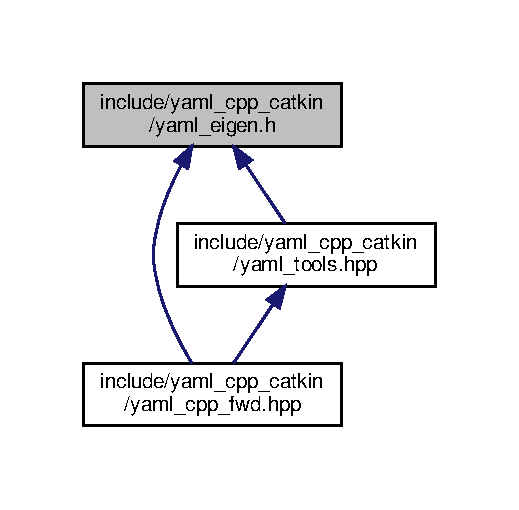
\includegraphics[width=249pt]{yaml__eigen_8h__dep__incl}
\end{center}
\end{figure}
\subsection*{Classes}
\begin{DoxyCompactItemize}
\item 
struct \hyperlink{structrobot__math_1_1MovableEigenVector}{robot\+\_\+math\+::\+Movable\+Eigen\+Vector$<$ T $>$}
\item 
struct \hyperlink{structrobot__math_1_1MovableEigenMatrix}{robot\+\_\+math\+::\+Movable\+Eigen\+Matrix$<$ T $>$}
\item 
struct \hyperlink{structYAML_1_1EigenVectorConverter}{Y\+A\+M\+L\+::\+Eigen\+Vector\+Converter$<$ Scalar, Rows, Cols, Align, Rows\+At\+Compile\+Time, Cols\+At\+Compile\+Time $>$}
\item 
struct \hyperlink{structYAML_1_1EigenMatrixConverter}{Y\+A\+M\+L\+::\+Eigen\+Matrix\+Converter$<$ Scalar, Rows, Cols, Align, Rows\+At\+Compile\+Time, Cols\+At\+Compile\+Time $>$}
\item 
struct \hyperlink{structYAML_1_1convert_3_01Eigen_1_1Matrix_3_01Scalar_00_01Rows_00_01Cols_00_01Align_00_01RowsAtC8665abb6da4eb6935869b0ee422ba9ce}{Y\+A\+M\+L\+::convert$<$ Eigen\+::\+Matrix$<$ Scalar, Rows, Cols, Align, Rows\+At\+Compile\+Time, Cols\+At\+Compile\+Time $>$ $>$}
\item 
struct \hyperlink{structYAML_1_1convert_3_01robot__math_1_1MovableEigenVector_3_01T_01_4_01_4}{Y\+A\+M\+L\+::convert$<$ robot\+\_\+math\+::\+Movable\+Eigen\+Vector$<$ T $>$ $>$}
\item 
struct \hyperlink{structYAML_1_1convert_3_01Eigen_1_1Quaterniond_01_4}{Y\+A\+M\+L\+::convert$<$ Eigen\+::\+Quaterniond $>$}
\end{DoxyCompactItemize}


\subsection{Detailed Description}
Add support for eigen frm the yaml-\/cpp standard package. 

\begin{DoxyAuthor}{Author}
Alexander Herzog 
\end{DoxyAuthor}
\begin{DoxyRefDesc}{License}
\item[\hyperlink{license__license000002}{License}]License B\+S\+D-\/3-\/\+Clause \end{DoxyRefDesc}
\begin{DoxyCopyright}{Copyright}
Copyright (c) 2019, New York University and Max Planck Gesellschaft. 
\end{DoxyCopyright}
\begin{DoxyDate}{Date}
2015-\/02-\/27 
\end{DoxyDate}

\hypertarget{yaml__tools_8hpp}{}\section{include/yaml\+\_\+cpp\+\_\+catkin/yaml\+\_\+tools.hpp File Reference}
\label{yaml__tools_8hpp}\index{include/yaml\+\_\+cpp\+\_\+catkin/yaml\+\_\+tools.\+hpp@{include/yaml\+\_\+cpp\+\_\+catkin/yaml\+\_\+tools.\+hpp}}
{\ttfamily \#include $<$yaml\+\_\+cpp\+\_\+catkin/yaml\+\_\+eigen.\+h$>$}\\*
Include dependency graph for yaml\+\_\+tools.\+hpp\+:
\nopagebreak
\begin{figure}[H]
\begin{center}
\leavevmode
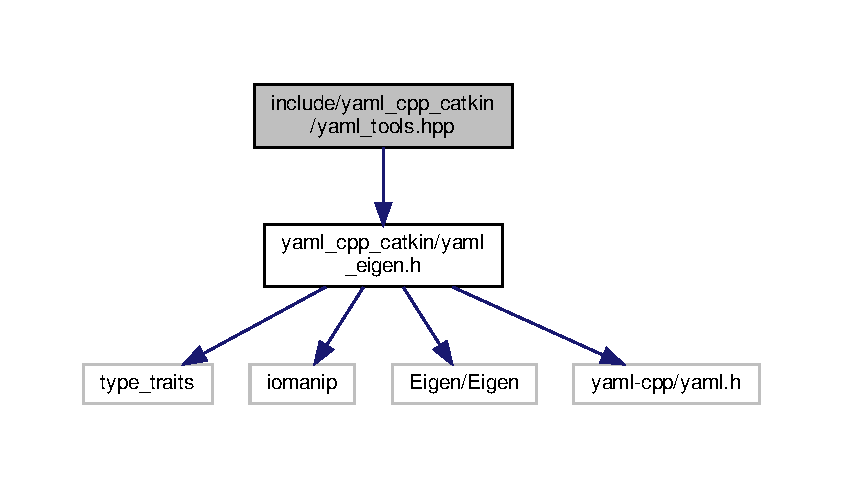
\includegraphics[width=350pt]{yaml__tools_8hpp__incl}
\end{center}
\end{figure}
This graph shows which files directly or indirectly include this file\+:
\nopagebreak
\begin{figure}[H]
\begin{center}
\leavevmode
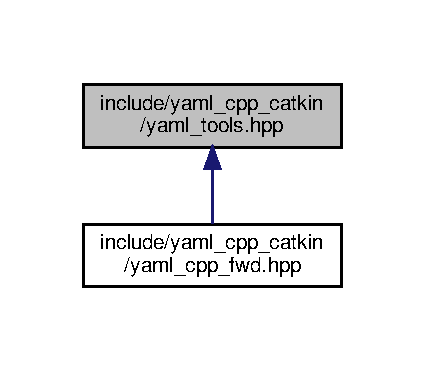
\includegraphics[width=204pt]{yaml__tools_8hpp__dep__incl}
\end{center}
\end{figure}
\subsection*{Functions}
\begin{DoxyCompactItemize}
\item 
{\footnotesize template$<$typename Yaml\+Type $>$ }\\static Yaml\+Type \hyperlink{yaml__tools_8hpp_aa37a27d8a4ee6a8ec1e16eb0208763e4}{Y\+A\+M\+L\+::\+Read\+Parameter} (const Y\+A\+M\+L\+::\+Node \&node, const std\+::string \&name)
\begin{DoxyCompactList}\small\item\em helper function to safely read a yaml parameter \end{DoxyCompactList}\item 
{\footnotesize template$<$typename Yaml\+Type $>$ }\\static void \hyperlink{yaml__tools_8hpp_a07d91dd29a0e49d11dac96037b626b20}{Y\+A\+M\+L\+::\+Read\+Parameter} (const Y\+A\+M\+L\+::\+Node \&node, const std\+::string \&name, Yaml\+Type \&parameter, bool optional=false)
\begin{DoxyCompactList}\small\item\em helper function to safely read a yaml parameter \end{DoxyCompactList}\item 
{\footnotesize template$<$typename Yaml\+Type $>$ }\\static void {\bfseries Y\+A\+M\+L\+::\+Read\+Parameter\+Default} (const Y\+A\+M\+L\+::\+Node \&node, const std\+::string \&name, Yaml\+Type \&parameter, Yaml\+Type default\+\_\+value)\hypertarget{yaml__tools_8hpp_a183f3b6513bd330027ea3c51d39161b5}{}\label{yaml__tools_8hpp_a183f3b6513bd330027ea3c51d39161b5}

\item 
{\footnotesize template$<$typename Yaml\+Type $>$ }\\void \hyperlink{yaml__tools_8hpp_a163f0c913b2e1d92245060b694dc25ad}{Y\+A\+M\+L\+::read\+Parameter} (const Y\+A\+M\+L\+::\+Node \&node, const std\+::string \&name, Yaml\+Type \&parameter, bool optional=false)
\begin{DoxyCompactList}\small\item\em helper function to safely read a yaml parameter \end{DoxyCompactList}\end{DoxyCompactItemize}


\subsection{Detailed Description}
\begin{DoxyAuthor}{Author}
Maximilien Naveau (\href{mailto:maximilien.naveau@gmail.com}{\tt maximilien.\+naveau@gmail.\+com}) 
\end{DoxyAuthor}
\begin{DoxyRefDesc}{License}
\item[\hyperlink{license__license000003}{License}]License B\+S\+D-\/3-\/\+Clause \end{DoxyRefDesc}
\begin{DoxyCopyright}{Copyright}
Copyright (c) 2019, New York University and Max Planck Gesellschaft. 
\end{DoxyCopyright}
\begin{DoxyDate}{Date}
2019-\/09-\/30 
\end{DoxyDate}


\subsection{Function Documentation}
\index{yaml\+\_\+tools.\+hpp@{yaml\+\_\+tools.\+hpp}!Read\+Parameter@{Read\+Parameter}}
\index{Read\+Parameter@{Read\+Parameter}!yaml\+\_\+tools.\+hpp@{yaml\+\_\+tools.\+hpp}}
\subsubsection[{\texorpdfstring{Read\+Parameter(const Y\+A\+M\+L\+::\+Node \&node, const std\+::string \&name)}{ReadParameter(const YAML::Node &node, const std::string &name)}}]{\setlength{\rightskip}{0pt plus 5cm}template$<$typename Yaml\+Type $>$ static Yaml\+Type Y\+A\+M\+L\+::\+Read\+Parameter (
\begin{DoxyParamCaption}
\item[{const Y\+A\+M\+L\+::\+Node \&}]{node, }
\item[{const std\+::string \&}]{name}
\end{DoxyParamCaption}
)\hspace{0.3cm}{\ttfamily [static]}}\hypertarget{yaml__tools_8hpp_file_aa37a27d8a4ee6a8ec1e16eb0208763e4}{}\label{yaml__tools_8hpp_file_aa37a27d8a4ee6a8ec1e16eb0208763e4}


helper function to safely read a yaml parameter 


\begin{DoxyTemplParams}{Template Parameters}
{\em Yaml\+Type} & \\
\hline
\end{DoxyTemplParams}

\begin{DoxyParams}{Parameters}
{\em node} & \\
\hline
{\em name} & \\
\hline
\end{DoxyParams}
\begin{DoxyReturn}{Returns}
Yaml\+Type 
\end{DoxyReturn}
\index{yaml\+\_\+tools.\+hpp@{yaml\+\_\+tools.\+hpp}!Read\+Parameter@{Read\+Parameter}}
\index{Read\+Parameter@{Read\+Parameter}!yaml\+\_\+tools.\+hpp@{yaml\+\_\+tools.\+hpp}}
\subsubsection[{\texorpdfstring{Read\+Parameter(const Y\+A\+M\+L\+::\+Node \&node, const std\+::string \&name, Yaml\+Type \&parameter, bool optional=false)}{ReadParameter(const YAML::Node &node, const std::string &name, YamlType &parameter, bool optional=false)}}]{\setlength{\rightskip}{0pt plus 5cm}template$<$typename Yaml\+Type $>$ static void Y\+A\+M\+L\+::\+Read\+Parameter (
\begin{DoxyParamCaption}
\item[{const Y\+A\+M\+L\+::\+Node \&}]{node, }
\item[{const std\+::string \&}]{name, }
\item[{Yaml\+Type \&}]{parameter, }
\item[{bool}]{optional = {\ttfamily false}}
\end{DoxyParamCaption}
)\hspace{0.3cm}{\ttfamily [static]}}\hypertarget{yaml__tools_8hpp_file_a07d91dd29a0e49d11dac96037b626b20}{}\label{yaml__tools_8hpp_file_a07d91dd29a0e49d11dac96037b626b20}


helper function to safely read a yaml parameter 


\begin{DoxyTemplParams}{Template Parameters}
{\em Yaml\+Type} & \\
\hline
\end{DoxyTemplParams}

\begin{DoxyParams}{Parameters}
{\em node} & \\
\hline
{\em name} & \\
\hline
{\em parameter} & \\
\hline
\end{DoxyParams}
\index{yaml\+\_\+tools.\+hpp@{yaml\+\_\+tools.\+hpp}!read\+Parameter@{read\+Parameter}}
\index{read\+Parameter@{read\+Parameter}!yaml\+\_\+tools.\+hpp@{yaml\+\_\+tools.\+hpp}}
\subsubsection[{\texorpdfstring{read\+Parameter(const Y\+A\+M\+L\+::\+Node \&node, const std\+::string \&name, Yaml\+Type \&parameter, bool optional=false)}{readParameter(const YAML::Node &node, const std::string &name, YamlType &parameter, bool optional=false)}}]{\setlength{\rightskip}{0pt plus 5cm}template$<$typename Yaml\+Type $>$ void Y\+A\+M\+L\+::read\+Parameter (
\begin{DoxyParamCaption}
\item[{const Y\+A\+M\+L\+::\+Node \&}]{node, }
\item[{const std\+::string \&}]{name, }
\item[{Yaml\+Type \&}]{parameter, }
\item[{bool}]{optional = {\ttfamily false}}
\end{DoxyParamCaption}
)}\hypertarget{yaml__tools_8hpp_file_a163f0c913b2e1d92245060b694dc25ad}{}\label{yaml__tools_8hpp_file_a163f0c913b2e1d92245060b694dc25ad}


helper function to safely read a yaml parameter 


\begin{DoxyParams}{Parameters}
{\em node} & \\
\hline
{\em name} & \\
\hline
\end{DoxyParams}

\begin{DoxyTemplParams}{Template Parameters}
{\em Yaml\+Type} & \\
\hline
\end{DoxyTemplParams}

\begin{DoxyParams}{Parameters}
{\em optional} & \\
\hline
\end{DoxyParams}
\begin{DoxyReturn}{Returns}
Yaml\+Type 
\end{DoxyReturn}

%--- End generated contents ---

% Index
\backmatter
\newpage
\phantomsection
\clearemptydoublepage
\addcontentsline{toc}{chapter}{Index}
\printindex

\end{document}
